\chapter{Virtualisierung}
\label{cha:virtualisierung}
Die Virtualisierung von IT-Systemen entwickelte sich in den letzten Jahren zur Standardlösung bei dem Betrieb von Server-Software, doch 2016 stagnierte der Erwerb von neuen Virtualisierungslizenzen zum ersten Mal.~\autocite{Gartner-Magic-Quadrant2016:online}
Zur Virtualisierung führte die Tatsache, dass leistungsfähigere Systeme, schnellere Technologiewechsel und sich ständig ändernde Voraussetzungen durch die Verwendung von rein hardwarebasierten Systemen zu teuer wurde.~\autocite{vmware-virtualization-history:online}

Warum Containertechnologien der nächste Schritt sind, welche Rolle Docker darin einnimmt und wohin diese Technologie noch führen kann, wird in diesem Kapitel erläutert.
\section{Beweggründe und Geschichte}
\label{sec:virtualisierungsgeschichte}
Im folgenden Absatz wird die Geschichte der Virtualisierung auf Basis von \autocite{Baun2009} kurz dargestellt.
In den 1960er-Jahren begann IBM mit dem Einsatz von Großrechnern, sogenannten Mainframes.~\autocite{IBM1981}
Da die Kosten für derartige Computersysteme den Einsatz eines einzelnen Rechners nicht gerechtfertigen konnten, wurden auf einem Mainframe mehrere Systeme parallel virtuell betrieben.
Dadurch konnte die Rechnenleistung effizienter ausgenutzt werden, sowie Versionsinkompatibiläteten durch den parallelen Betrieb alter und neuer Mainframes vermieden werden.
Als im Laufe der 80er-Jahre die x86-Architektur den Aufschwung erlebte, stand die Virtualisierung still.
Der günstige Preis und die fehlende Virtualisierungsunterstützung machten es unnötig und unmöglich Endgeräte zu virtualisieren.
Erst mit der wieder steigenden Rechenleistung und des Erscheinens von Mehrkernprozessoren hat die IT-Virtualisierung wieder an Traktion gewonnen.
In den letzten Jahren wird besonders durch Cloud-Angebote alles Mögliche nur mehr virtuell betrieben.
Von der  kompletten Netzwerkinfrastruktur, bis hin zum Speicher wird in modernen Rechenzentren (Amazon Web Services\footnote{\url{https://aws.amazon.com/}}, Microsoft Azure\footnote{\url{https://azure.microsoft.com/}}, \dots) alles virtualisiert.
Die Analyse-Firma Gartner Inc.\ spricht von einem Virtualisierungsgrad von 75\% im Serverbereich \autocite{Gartner-Server-Virtualization:online}.
Aspekte wie die einfache Provisionierung von virtualisierten Systemen führen dazu, dass beispielsweise eine horizontale Skalierung ohne großen Mehraufwand betrieben werden kann.
Auch das Testen von Infrastrukturen wurde durch Virtualisierung ermöglicht.
Es ist nicht mehr notwendig ein gesamtes IT-System temporär lediglich zu Testzwecken zur Verfügung zu stellen, oder sogar ein solches eigenes anzuschaffen, stattdessen können die benötigten Ressourcen in der Cloud lediglich für den benötigten Zeitraum angemietet werden.
% TODO: evtl. Warum wird heutzutage virtualisiert (Cloud-Umgebungen, Skalierung, Ressourcenverteilung) + Gartner-Trends

Zahlreiche Vorteile der Virtualisierung, führten im Gegensatz zu den wenigen Nachteilen zur großen Adaption und Verbreitung.
\subsubsection{Vorteile der Virtualisierung \autocite[198]{Baun2009}}
Der kostensparendste Aspekt der Virtualisierung ist die Konsolidierung von Servern.
Server, die nicht unter voller Last laufen, benötigen trotzdem Strom, Kühlung, Wartung und Infrastruktur.
Durch Konsolidierung können nun ungenutzte Ressourcen genutzt werden, die zuvor lediglich Kostern verursachten.
Virtualisierte Server bieten sind außerdem erheblich einfacher zu provisionieren.
Wird ein neuer Server benötigt, können dazu bestehende, freie Ressourcen genützt werden, anstatt, dass weitere Hardware anzuschaffen ist.

Wartungsaufgaben werden stark vereinfacht, da durch diverse Managementwerkzeuge viele Aufgaben automatisiert, sowie ohne einer Änderung an den physischen Systemen durchgeführt werden können.
Dazu zählt auch die Live-Migration von virtuellen Maschinen.
Diese können dadurch für den Endanwender unterbrechungsfrei und daher unbemerkt zwischen zwei Rechnern verschoben werden.
So wird Wartung an der Hardware ermöglicht, ohne dass sich eine Downtime für die Benutzer ergibt, Voraussetzung dafür ist allerdings, dass Ressourcen im Rechenzentrum frei sind, auf die Systeme (temporär) migriert werden können.

Durch Virtualisierung wird auch die Dimensionierung der Ressourcen erheblich vereinfacht, da lediglich eine ungefähre Menge an Rechenleistung initial zu schätzen ist, diese sich allerdings im Betrieb umverteilen lässt.
So können Systeme, die ihre Leistungsgrenzen erreicht haben, oder bei weitem nicht nützen im laufenden Betrieb neu dimensioniert werden.
Dazu kommt die vorhin beschriebene Live-Migration zum Einsatz.
Laut \autocite{Hantelmann2008} können die Rechenzentrumskosten um 50\% reduziert werden, wohingegen die Anschaffungskosten neuer Hardware um bis zu 70\% verringert werden können.
\autocite{Azure-Scaling:online} beschreibt Möglichkeiten zur automatischen Skalierung von Ressourcen in der Microsoft-Azure-Cloud.
Dabei spielt Virtualisierung eine essentielle Rolle, da alle bei Azure gemieteten Ressourcen virtualisiert laufen.
So kann in diesem Fall allerdings eine, für den Systemadministrator, angenehme Version der Dimensionierung erreicht werden, da die Azure-Cloud automatisch die Leistung der Ressourcen an die aktuelle Auslastung anpasst.

Nicht nur durch Features wie die Live-Migration wird die Flexibilität in virtualisierten Rechenzentren erhöht.
Virtuelle Maschinen bestehen aus wenigen Dateien, von denen sehr einfach Klone zum Backup erstellt werden können.
Zusätzlich gibt es die Funktion von Snapshots, dabei wird ein Abbild einer virtuellen Maschine erstellt, das jederzeit wieder hergestellt werden kann.
Dies ist besonders hilfreich, wenn es Snapshots von fertig konfigurierten, jedoch unbenutzten Systemen gibt, da damit fehlerhafte Maschinen sehr schnell wieder hergestellt werden können.

Durch die Abschottung der virtuellen Maschinen gegeneinander können trotz der Virtualisierung hohe Service Level Agreements erreicht werden, da der Ausfall einer Maschine lediglich diese betrifft, das Hostsystem bleibt allerdings intakt.
In einem Hochverfügbarkeitsszenario besteht auch die Möglichkeit, dass ein überwachendes System (Supervisor) den Ausfall erkennt und solch ein System auf einem anderen Knoten neu startet.

\subsubsection{Nachteile der Virtualisierung \autocite[198]{Baun2009}}
Da bei virtualisierten Systemen die Instruktionen auf vom virtuellen auf das Hostsystem umgesetzt werden müssen, ergibt sich ein Leistungsverlust.
Dieser wird allerdings mit leistungsfähigeren Mehrkernprozessoren und durch Prozesservirtualisierung wie Intel® VT\footnote{\url{http://www.intel.de/content/www/de/de/virtualization/virtualization-technology/intel-virtualization-technology.html}} verschwindend gering.
Die Prozessoren bieten native Virtualisierungstechniken an, bei denen die Befehle nicht mehr umgesetzt werden müssen, wodurch die Verringerung der Leistung auf unter 10\% \autocite{Hardt2005} sinkt.

Ein wesentlich größeres Problem in der Virtualisierung stellen besondere Hardwareanforderungen dar.
Authentifizierung über Hardware-Dongles oder die Ansteuerung von Legacy-Hardware ist in virtualisierten Umgebungen durch den fehlenden Direktzugriff auf die Hardware sehr schwierig bis nicht möglich.

Besondere Vorsicht muss außerdem der Infrastruktur in den Rechenzentren zukommen, da bei einem Hostausfall in virtualisierten Umgebungen zahlreiche Systeme betroffen sind.
Dieses Problem lässt sich durch redundante Installationen und gut durchdachte Ausfallkonzepte lösen, wobei hier die Vermeidung eines \emph{Single Point of Failures} (SPOF) höchste Priorität genießen muss.
Damit ein redundantes System im Fehlerfall Wirkung zeigen kann, muss dieses vollredundant sein.
Die Konzeption, Installation und der Betrieb eines solchen Systems erfordern eine hochwertige Infrastruktur und zusäzliches Detailwissen.


\section{Vollvirtualisierung}
\label{sec:vollvirtualisierung}
\autocite{Baun2009} stellt dar, dass die Vollvirtualisierung Gastsystemen eine gesamte virtuelle Umgebung zur Verfügung stellt.
Weiters wird darin das Zusammenspiel der einzelnen Komponenten folgendermaßen beschrieben.
Der \emph{Virtuelle Maschinenmonitor} (VMM) läuft auf dem Host-System und ist jene Komponente, die die virtuelle Umgebung zur Verfügung stellt.
Dieses vollwertige System beinhaltet ein BIOS, sowie eine Abstraktion der gesamten Hardware, wodurch die Gast-Systeme nicht merken, dass sie virtualisiert werden.
Zugriffe auf die Hardware werden vom VMM intelligent auf die Hardware des Hosts verteilt, oder über Hardware-Emulation zugänglich gemacht.
Dieser Aufbau ist in \cref{fig:architektur-vollvirtualisierung} zu sehen.
\begin{figure}[htbp]
    \centering
    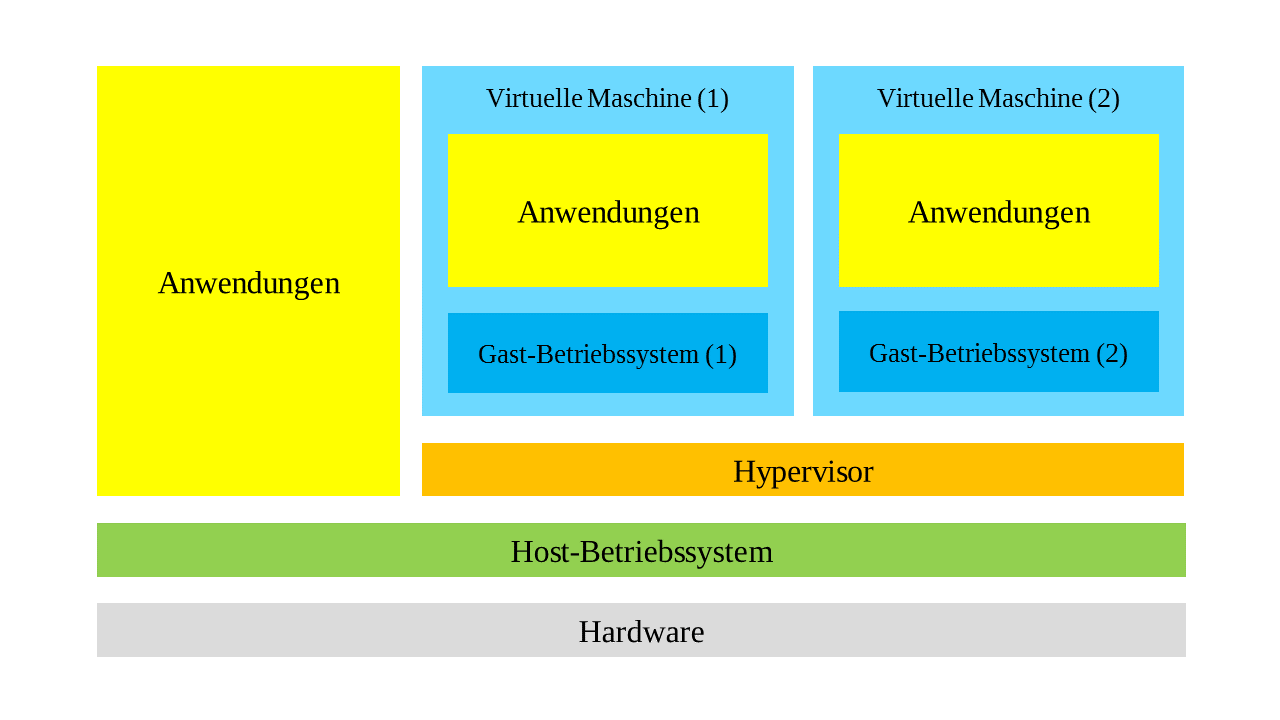
\includegraphics[width=0.9\linewidth,clip]{images/vollvirtualisierung}
    \caption{Architektur der Vollvirtualisierung}
\label{fig:architektur-vollvirtualisierung}
\end{figure}
Einerseits zeigt die Abbildung, dass Anwendungen ohne Problem parallel zu den virtualisierten Systemen laufen können, andererseits wird verdeutlicht, dass jedes virtuelle System ein gesamtes Betriebssystem (Gast-OS) beinhaltet.
Jegliche Kommunikation eines Gastsystems mit den Systemresourcen des Hosts läuft über den VMM, wodurch gewährleistet wird, dass dieser Zugriff kontrolliert werden kann.
Dies stellt sicher, dass die virtuellen Maschinen voneinander abgeschottet sind und ein Ausfall eines Gastsystems die anderen nicht beeinflusst.

Aus dieser hohen Abstraktion folgt, dass am Gastsystem keine Änderungen durchgeführt werden müssen und unterschiedliche Kernels parallel virtualisiert werden können.
Lediglich die Prozessorarchitektur muss zusammenpassen.
Der Vorteil eines gesamten Betriebssystems pro Gastsystem bringt allerdings den Nachteil mit sich, dass jedes dieser Systeme Speicher für den Kernel und das Betriebssystem belegt. Weiters ist ein Bootvorgang nötig, der die Verwendung zu Entwicklungszwecken verzögert.
Allerdings gibt die Vollvirtualisierung dem Entwickler die Möglichkeit, seine Software auf dem lokalen Rechner auf verschiedenen Betriebssystemen zu testen, oder Werkzeuge zu verwenden, die auf dem Host-System nicht verfügbar sind.
Außerdem können vorgefertigte \emph{Basissysteme} (Snapshots) für die Entwickler bereitgestellt werden, um die Konfigurationszeit zu verkürzen und eine einheitliche Entwicklungsumgebung zu haben.
Folgende Probleme treten hingegen in einer virtualisierten Entwicklungsumgebung auf:
\begin{itemize}
\item Updates müssen nun entweder doppelt durchgeführt werden, oder die Entwickler werden periodisch mit neuen Snapshots versorgt.
\item Für die Daten und Konfigurationen der Entwickler muss ein Platz außerhalb der virtuellen Maschine gefunden werden. Besonders bei einem Snapshot-basierten Updateverfahren gehen durch die Verwendung eines neuen Snapshots alle Daten in der VM verloren. Die Konfiguration der Entwicklungsumgebung können idealerweise auf Netzwerklaufwerke verlegt werden und die Quelltexte sollten sich in einem Versionskontrollsystem befinden.
\item Ein weiters Problem mit den Daten betrifft die Authentifizierung. Für SSH-Schlüssel für Versionskontrollsysteme und andere Zugangsdaten muss ebenfalls eine Möglichkeit geschaffen werden, diese in die virtuellen Maschinen zu bringen.
\item Entwicklungsumgebungen gelangen bei virtualisierten System schnell an die Performancegrenzen, wodurch die Produktivität der Mitarbeiter sinkt.
\item Bei mehreren parallelen Projekten und damit verbundenen virtuellen Maschinen kann der Speicherplatz auf dem Host-System sehr knapp werden.
\end{itemize}
Wie sich die Vollvirtualisierung für Entwickler in der Praxis verwenden lässt, wird in \cref{sub:vagrant} dargestellt.

% TODO: evtl. Gartner Servervirtualisierung
% - http://www.gartner.com/newsroom/id/3315817
% - https://www.gartner.com/doc/reprints?ct=160707&id=1-3B9FAM0&st=sb
\section{Containervirtualisierung}
\label{sec:containervirtualisierung}
Die Containervirtualisierung, auch manchmal Betriebssystemvirtualisierung genannt, bringt lediglich ähnliche Ergebnisse hervor als die Vollvirtualisierung, hat allerdings eine fundamental andere Funktionsweise.
Der folgende Absatz baut auf \autocite{EntwicklerDE2015} auf, worin ein sehr guter Überblick über die Funktionsweise der Containervirtualisierung gegeben wird.
In \cref{fig:architektur-containervirtualisierung} ist die wesentlich schlankere Architektur der Containervirtualisierung zu sehen.
\begin{figure}[htbp]
    \centering
    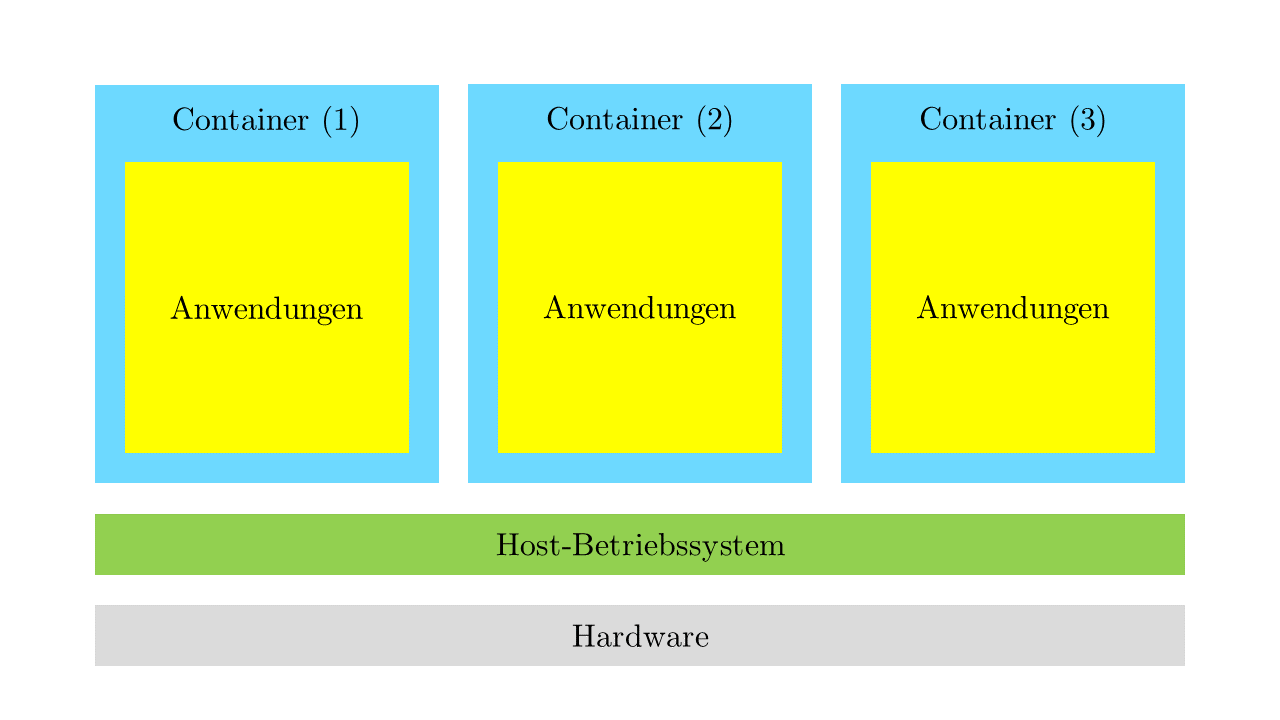
\includegraphics[width=0.9\linewidth,clip]{images/containervirtualisierung}
    \caption{Architektur der Containervirtualisierung}
    \label{fig:architektur-containervirtualisierung}
\end{figure}
Darin fällt auf, dass es zwischen dem Host-Betriebssystem und den Containern keine Zwischenschicht gibt.
Im Fall der Containervirtualisierung ist der Host gleichzeitig Hypervisor, wodurch eine Virtualisierung mit einem wesentlich geringeren Overhead entsteht.
In manchen Grafiken zur Containervirtualisierung existiert eine Schicht zwischen dem Host und den Containern, welche allerdings lediglich darstellt, dass die Container irgendwie gestartet werden müssen, tatsächlich wird eine abgeschottete Instanz des Host-Betriebssystems erzeugt, aus der die Anwendungen nicht ausbrechen können.
Ein weit verbreitetes Synonym ist \emph{Jails}, basierend auf dem Namen dieser Funktion in BSD\footnote{\url{https://www.freebsd.org/doc/de_DE.ISO8859-1/books/handbook/jails.html}}.

Diese Funktionsweise wird in \autocite{Diedrich2016} beschrieben.
Jede virtualisierte Instanz bekommt eine eigene Sicht auf den Kernel und dessen Funktionen, die aber strikt von den anderen virtualisierten Instanzen getrennt ist.
So ist keine Vollvirtualisierung notwendig, da Betriebssystemfunktionen direkt vom Kernel verarbeitet werden.
Dies führt zu der bei Containern üblichen extrem schnellen Startzeit.
Da die Virtualisierung über eine geteilte Kernel-Instanz abgewickelt wird, besteht bei der Containervirtualisierung die Einschränkung, dass das Gast-System den gleichen Kernel unterstützen muss, wie das Hostsystem.
Für diese abgeschottete Instanz des Betriebssystems sind folgende zwei Funktionen aus dem Linux-Kernel notwendig:
\begin{description}
    \item [namespaces] Namespaces sind die Grundlage für die Abschottung der Prozesse untereinander. Diese Namensräume ermöglichen es Prozessen, dass sie private \emph{Prozess-IDs} (PIDs) verwalten. Diese Prozesse und ihre Kinder können nun die anderen PIDs nicht sehen, wodurch eine Abstraktion erreicht wird, die einer Virtualisierung ähnelt.
    \item [cgroups] Durch Namensräume wird zwar das Problem der Abschottung gelöst, allerdings können sich Prozesse gegenseitig stören, da sie keine Limits bei der Verwendung ihrer Ressourcen auferlegt bekommen. \emph{Control Groups} (cgroups) lösen genau dieses Problem, sie erlauben eine Zuteilung von RAM, CPU-Zeit und Disk-I/O zu einzelnen Prozessen. So können sich Prozesse gegenseitig keine Ressourcen wegnehmen, es entsteht allerdings kein Overhead, da nativ am Kernel gearbeitet wird.
\end{description}
Das oft erwähnte \emph{LXC\footnote{https://linuxcontainers.org/}} (Linux Containers) verwendet \emph{namespaces} und \emph{cgroups} zum Erstellen und Verwalten von Containern, wurde früher von vom Container-Marktführer Docker verwendet, zwischenzeitlich allerdings durch \emph{libcontainer} ersetzt und nun durch \emph{runc\footnote{https://runc.io/}} abgelöst.
Dies ist nun in der \emph{Open Container Initiative} (OCI, siehe \cref{sec:open-container-initiative}) standardisiert.
Die hier beschriebene Containervirtualisierung trifft lediglich auf die Linux-Container zu. Microsoft arbeitet gerade an einer ersten Versioin der Windows Container\footnote{https://docs.microsoft.com/en-us/virtualization/windowscontainers/about/}, leitet diesen Artikel allerdings mit "This is preliminary content and subject to change." ein, weshalb diese Technologie aufgrund des Erscheinungsdatums aus dieser Arbeit ausgeklammert wurde.

% - https://semaphoreci.com/community/tutorials/how-to-deploy-a-go-web-application-with-docker

\subsection{Implementierungen von Containervirtualisierungslösungen}
Für das Verwalten und Starten von Containern gibt es zahlreiche Lösungen, wobei \autocite{rkt-comparison:online} einen Vergleich dieser bietet.
\label{sec:container-solutions}
\begin{description}
    \item [Docker] Da Docker die in dieser Arbeit verwendete Technologie ist, wird sie in \cref{cha:docker} ausführlich behandelt und die Verwendung exemplarisch gezeigt.
    \item [rkt] rkt (ausgesprochen: rocket) ist ein Container-Manager des quelloffenen Unix-Systems CoreOS. Im Gegensatz zu Docker ist es lediglich ein einzelnes ausführbares Programm ohne Hintergrundprozess (Deamon). Die Images der Container werden über HTTPS verteilt. Durch den fehlenden Deamon kann rkt sehr einfach in bestehende Systeme wie systemd und Kubernetes integriert werden. rkt baut auf dem standardisierten Containerformat appc\footnote{https://github.com/appc/spec/} auf.
    \item [runc] runc ist eine sehr systemnahe Möglichkeit Container zu starten und zu verwalten. Sie bietet allerdings keine Möglichkeit Images herunterzuladen und erfordert hohe Detailkenntnisse des Betriebssystems und dessen Konfiguration.
    \item [containerd] containerd ist ein Deamon für runc. Auch hier ist keine Möglichkeit für den Download von Images vorhanden. containerd und runc bieten die Basis für Docker seit der Version 1.11.0.
    \item [LXC] Der primäre Einsatzzweck von LXC ist das Starten einer kompletten Linux-Version parallel zum Host-System. Anwendungscontainer können auch verwaltet werden, erfordern allerdings mehr Wissen als zum Beispiel mit Docker oder rkt.
\end{description}
% - file:///D:/download/Realitaetscheck-Brauchen-wir-Docker-wirklich_Nils-Magnus_inovex-GmbH.pdf
\subsection{Open Container Initiative (\emph{OCI})}
\label{sec:open-container-initiative}
Um einen industrieweiten Standard für Container zu erstellen, hat Docker auf der DockerCon 2015 die damals noch Open Container Project genannte Initiative unter der Linux Foundation vorgestellt.~\autocite{docker-ocp:online}
Die OCI beschreibt mit \autocite{oci-about:online} spezifiziert folgende zwei Standards:
\begin{description}
    \item [runtime-spec\footnote{https://github.com/opencontainers/runtime-spec}] Die Runtime-Spezification regelt wie ein bereits entpackter Container (Filesystem Bundle) ausgeführt wird.
    \item [image-spec\footnote{https://github.com/opencontainers/image-spec}] Das Ziel der Image-Specification ist ein Format zu definieren, das das erstellen, verifizieren, benennen und verteilen von Images ermöglicht.
\end{description}
Der Inititative sind mittlerweile zahlreiche große Unternehmen beigetreten um Containertechnologien zu standardisieren. Einige davon sind: Amazon, Cisco, Docker, Facebook, Hewlett Packard, IBM, Intel und Microsoft.\footnote{https://www.opencontainers.org/about/members}

\subsection{Orchestrierungssysteme}
\label{sec:orchestrierungssysteme}
Im Folgenden werden kurz die aktuell wichtigsten Orchestrierungssysteme für Container und deren Zweck beschrieben.
Softwareentwickler werden diese weder lokal zur Entwicklung benötigen, noch aktiv in der Produktion einsetzen, doch ein kurzer Überblick ist aus drei Gründen sehr wichtig.
Die Entwickler sollten zumindest wissen, was Orchestrierung ist und warum es notwendig ist.
Außerdem fallen diese Schlagwörter beim Arbeiten mit Containern sehr oft. Ein Basiswissen dazu genügt, um zu entscheiden, ob das vorgeschlagene Werkzeug im konkreten Problemfall wirklich relevant ist.
Die Funktionsweise und Philosopohie der Containerorchestrierung sollte schon im Entwicklungsprozess bedacht werden, da die Architektur von Anwendungen davon stark beeinflusst wird.
Das Wissen über die Behandlung von Containern verhindert Fehler beim Programmieren und zwingt die Entwickler auch an den Betrieb der Software zu denken, wodurch die Idee des \emph{DevOps} in den Entwicklungszyklus integriert wird.

Die Orchestrierung von Containern kann auch als Besetzung bezeichnet werden, wobei den jeweiligen Aufgaben in einem Softwaresystem mithilfe von Containern Services zugewiesen werden.
Diese Zuteilung geschieht deklarativ, wodurch gleichzeitig eine skalierbare Konfiguration entsteht.
Das Orchestrierungssystem weiß nun welche Container es für welchen Zweck einsetzen muss und wie diese skaliert werden sollen. An dieser Stelle wird meistens Cattle vs. Pet-Analogie verwendet.~\autocite{pets-vs-cattle:online}
In containerbasierten Systemen werden die Serviceinstanzen nicht als Pets angesehen, um die sich der Administrator händisch kümmern muss und alles versucht um sie am Leben zu erhalten.
Stattdessen werden die Container als Herde betrachtet, bei der der Ausfall eines Services durch die große Menge kompensiert wird.
Außerdem ist das System so gebaut, dass das Orchestrierungswerkzeug den Ausfall eines Containers erkennt und einfach einen neuen Container dieser Art startet und konfiguriert.
Die Folge dieser Philosophie ist, dass das Softwaresystem so gebaut werden muss, dass es auch den Ausfall und womöglich häufigen Neustart einzelner Servies verkraftet.

\autocite{ix-orchestrierung-2017} liefert einen Überblick über die aktuell am meisten verwendeten Werkzeuge zur Containerorchestrierung.
\begin{description}
    \item [Kubernetes] Wenn es um die Verwaltung von sehr vielen Containern (mehrere Tausende) geht, dann ist der Cluster-Manager Kubernetes von Google das Richtige. Die Archtitektur ist nach dem Master/Slave-Schema aufgebaut. Der Master verteilt die Arbeit auf zahlreiche Knoten. Die Container werden noch einmal abstrahiert, indem sie zu sogenannten Pods zusammengefasst werden. Kubernetes wird über die Kommandozeile konfiguriert, wodurch es Einsteiger mit einer sehr steilen Lernkurve konfrontiert.
    \item [DC/OS] DC/OS ist ein Cluster-Manager, der in der Cloud laufen kann. Er kann außerdem nicht nur Container verwalten, sondern auch benutzerdefinierte Pakete. Durch diese Flexibilität ist DC/OS sehr komplex, besitzt jedoch eine automatische Installation und eine grafische Benutzeroberfläche. Zu großer Verwirrung können die verwendeten Namen führen. DC/OS steht für "Datacenter Operating System". Ein Teil von DC/OS heißt Mesos und die Software selbst ist von der Firma Mesosphere.
    \item [Rancher] Rancher ist ein Orchestrierungsprodukt der Firma RancherOS. Genau wie Kubernetes ist die Architektur aufgeteilt in einen Master und mehrere Agenten. Rancher selbst ist ein Docker-Container, der beim Starten privilegierte Rechte erhält um selbst wieder Container starten zu können. Rancher erweitert die bestehenden Docker-Componenten, verwendet allerdings dieselbe Syntax, wodurch ein schneler Einstieg ermöglicht wird.
    Zusätzlich gibt es für die Verwaltung eine grafische Benutzeroberfläche. Wenn die Anwendung über die Möglichkeiten von Rancher hinauswächst, bietet Rancher an, Kubernetes oder Mesos zu integrieren und Rancher lediglich als Verwaltungswerkzeug dessen zu verwenden.
\end{description}
% - DC/OS
% - Mesosphere
% - Swarm
% - Kubernetes
% - https://www.sigs-datacom.de/uploads/tx_dmjournals/rossbach_OTS_Architekturen_15.pdf !!!
% - https://www.google.at/search?q=container+orchestration&ie=&oe=
% - http://stackoverflow.com/questions/29198840/marathon-vs-kubernetes-vs-docker-swarm-on-dc-os-with-docker-containers
